\begin{center}
\section{緒論}
\end{center}

\subsection{背景}
近年來數據以飛快的速度成長,TB或是PB等級的數據隨處可見。在這資料快速產生且數據快速交換的時代,大數據一詞也常被提及。國際數據公司(International Data Corporation, IDC)有研究指出\cite{gantz2011extracting},在2011年,創建和複製的資訊量以及資料量將超過1.8 ZB。這麼龐大的資料也成了產業界與學術界所需要探討的重要議題。而有這麼大量的資料也意味著會有大量的應用產生,而這一些應用當中一定會需要資料的交換,而在交換資料的時候,大多數的應用會選擇XML。\\\par
在大數據中常使用5V\cite{ibm5v}\cite{khan2014big}來描述大數據的特性。所謂的5V是指Volume、Vleocity、Variety,、Value以及Veracity。Volume是指產生的資料量;Velocity是指資料產生的速度;Variety是指資料的多樣性;Value是指資料的價值;Veracity\cite{veracityimpor}是指資料的可信度或是真實度。而大數據在做資料交換的時候我們所關心的是資料的可信度或是真實度,也就是上述所提到的Veracity,這會影響到我們在做資料分析的結果可信度。假使進來的資料不具可信度的話,那麼所分析出來的結果自然也就不具有任何價值。本研究基於Apache Spark建構XML Veacity 真實度模型,利用Apache Spark 分散式大數據處理引擎,來計算並建構大型XML文件的Veracity 模型,並且將此模型應用在串流XML文件的Veracity 真實度評分。

\subsection{XML}
可延伸標記式語言(Extensible Markup Language,簡稱XML)\cite{rfc7303},是一種作為資料交換的結構化資料格式。XML是從標準通用標記式語言(SGML)中簡化修改出來的。XML是從1995年開始有雛形,並向全球資訊網聯盟(World Wide Web Consortium,簡稱W3C)提案,而在1998年2月發布為W3C的標準(XML 1.0)。\\\par
XML的特色在於文件內的標籤名稱可以由使用者自行定義,而XML文件必須是結構完整的(well-formed)。所謂的well-formed是指XML要符合每一個標籤都要有起始元素之巢狀結構,而符合格式規範,如DTD或XML Schema得則稱為有效的XML(Valid XML)。在XML中我們為了確保文件的格式正確性,會使用DTD(Document Type Definition)\cite{dtd}或是XML Schema\cite{xsd}。DTD是XML提供的文件驗證機制,這是用來定義文件合法區塊,也就是定義元素的架構,有使用DTD的XML都必須依照DTD所定義的格式來呈現。圖\ref{xml1}是一個使用DTD且well-formed的XML文件,在圖\ref{xml1}當中的第2行到第8行即是DTD驗證的格式。從第2行開始宣告了這一份XML文件的根節點(root),再來第3行宣告了根節點下有哪一些子節點,第4行到第7行宣告了子節點下皆為資料,沒有接續的子節點。

\begin{figure}[H]
\centering
\graphicspath{{/Users/FUDA/Documents/masterThesis/image/}}
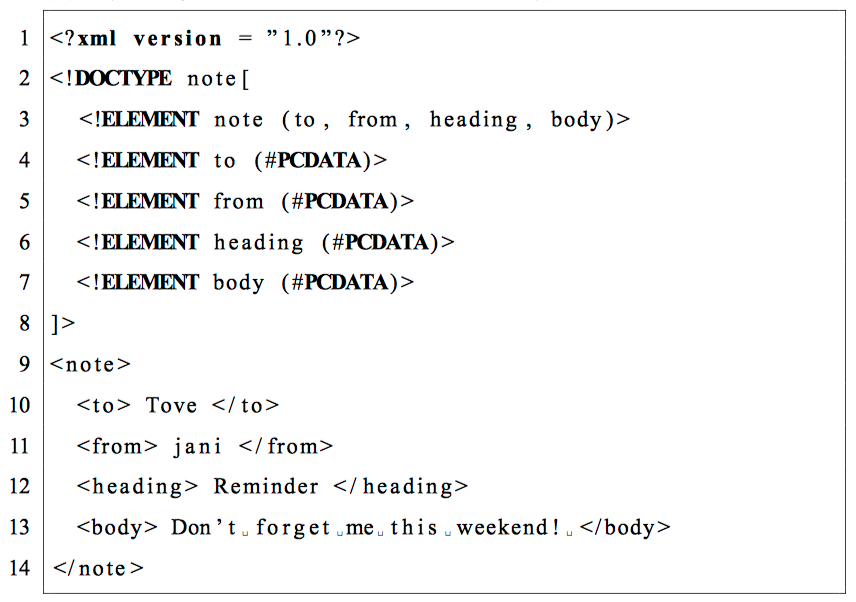
\includegraphics[scale=0.5]{xml1.png}
\caption{example1.xml}
\label{xml1}
\end{figure}

但由於XML DTD並不能完全滿足XML自動化處理的要求,也缺乏對於文件結構屬性和資料屬性的規範。所以W3C在2001年的時候提出XML Schema。XML Schema使用的語法與XML相同,且支援多種資料類型。圖\ref{xml2}是一個使用XML Schema 驗證的XML文件,在圖\ref{xml2}的第4行即宣告了XML Schema的路徑位置,而XML Schema的格式如圖\ref{schema}所示,且可以看到在語法的部分與XML相同採用巢狀的結構。而XML Schema與DTD的不同之處在第5行到第10行,XML Schema對於每一個節點有著更詳細的資料型態定義,在語法以及文件結構上面也更趨近於XML。\\\par

\begin{figure}[H]
\centering
\graphicspath{{/Users/FUDA/Documents/masterThesis/image/}}
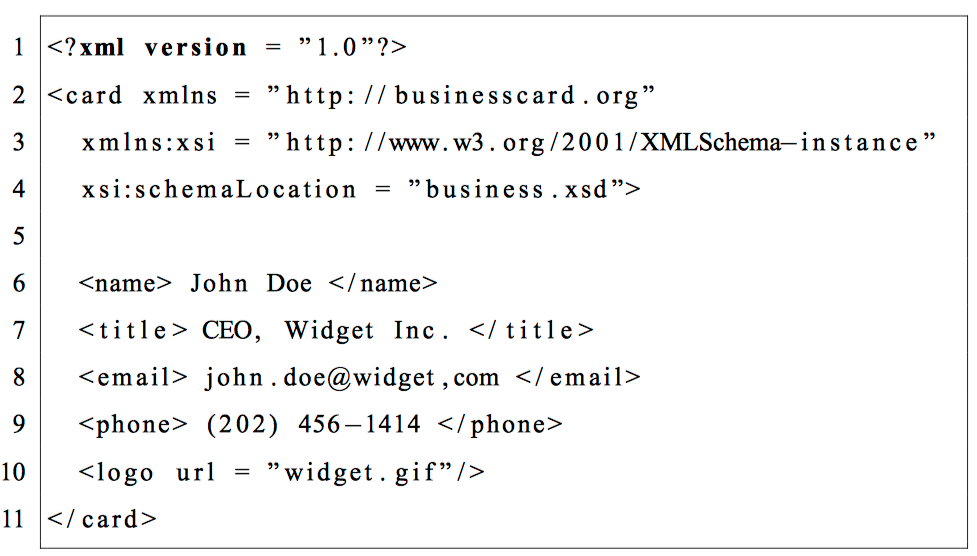
\includegraphics[scale=0.4]{xml2.png}
\caption{example2.xml}
\label{xml2}
\end{figure}

\newpage

\begin{figure}[H]
\centering
\graphicspath{{/Users/FUDA/Documents/masterThesis/image/}}
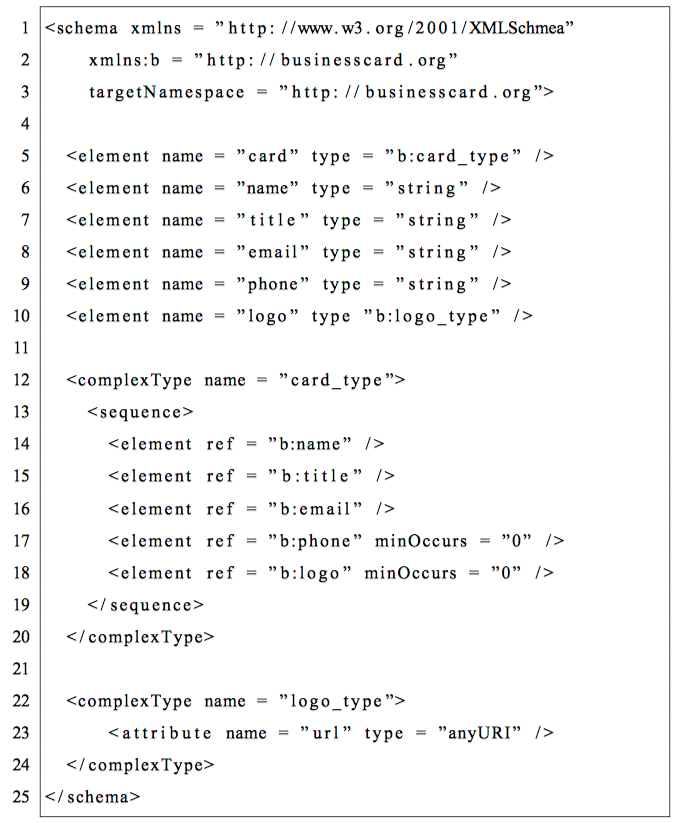
\includegraphics[scale=0.55]{schema.png}
\caption{XML Schema}
\label{schema}
\end{figure}
\newpage
\newpage
\subsection{Apache Spark}
為了解決大數據的計算問題,在2008年的時候Google提出了MapReduce\cite{mapreduce}的運算框架,用於大數據的處理。MapReduce是由Map和Reduce所組成的,Map的動作是將大的計算任務切割成小任務來操作,Reduce是將前面Map切出來並算完的小任務做合併,來取得最終的結果。後來這樣的一個計算框架演變成我們現在所熟悉的Hadoop\cite{hadoopwebsite}。\\\par
在2010年Yahoo提出了HDFS(Hadoop Distributed File System)\cite{hdfs}來解決大數據資料儲存的問題。HDFS為一個分散式檔案儲存系統,將單一檔案切割成數份,分別複製以及儲存到叢集節點當中,以達到儲存的目的。而這樣的的系統好處有三點:第一點為可擴展性(Data Scalability),當叢集的儲存空間不足的時候可以非常輕易的做擴充;第二點為容錯性(Fauit Tolerance):當其中一個儲存節點內資料有損壞的時候,系統可以從其他節點找到遺失的資料切片的備份來還原資料本身;第三點為並行性(High Concurrency):藉由分散式檔案系統可以讓資料並行處理。然而Hadoop有一個缺點,在進行MapReduce的時候,每一次的計算都是需要硬碟的I/O。這樣的行爲造成了效能的瓶頸。所以有了新一代的運算框架。\\\par
Apache Spark\cite{sparkwebsite}為一個開源的大數據分散式引擎,最初是2009年由加州大學柏克萊分校AMPLab所提出,為記憶體內(In-memory)的計算。跟Hadoop相比,Apache Spark 的計算效率比起Hadoop來說有顯著的提升,其原因為Apache Spark在運算的時候,將運算中間產生的資料暫存在記憶體中,因此可以加快整體運行速度,而Hadoop則是在每一次計算完成或是產生中間資料的時候,都必須對硬碟動作,這個動作降低了Hadoop的執行效率,而Apache Spark的設計則能夠增加計算的效率。除了上述提到的效能問題之外,Hadoop只支援Map和Reduce這兩種運算,對於現今要處理的資料來說,在撰寫程式的時候靈活度不夠,而且MapReduce在運行任務的時候,任務排程以及啟動開銷大,基於上述原因,Apache Spark是目前較好的大數據處理引擎。\\\par

Apache Spark主要的對資料的操作是使用叫做RDD(Resilient Distributed Datasets,彈性分佈資料集)\cite{zaharia2012resilient},RDD的結構如圖\ref{rdd}所示。RDD是具有容錯機制以及高效能的抽象資料結構。在圖\ref{rdd}中黃色的區塊是RDD當中所謂的Partition,是指資料的分片。一個RDD會由一個到多個的Partition所組成,程式在運行的時候,Parttion會分散至各叢集節點當中進行運算,會存放在記憶體內,所以可以快速分享各個Partition的運算結果。RDD是一個可以並列操作且有容錯機制的資料集合。且可以透過參照外部儲存系統的資料集建立,或者是透過現有的RDD轉換而創建,例如map, join, reduce等對於資料的操作,而在Apache Spark 對於RDD的操作中,有分為轉換(Transformation)和動作(Action),Apache Spark 在做資料操作的時候,採用的是惰性求值,也就是當Apache Spark 在做 Transformation的時候,並不是馬上會做資料的轉換,而是會先把要轉換的動作記錄下來,等到有呼叫Action的API的時候才會依照剛才做資料的操作並輸出結果,這樣可以使執行效能提高,例如一個資料經過 MapReduce處理後會得到一個結果,而不是返回一個大的資料集。
\begin{figure}[H]
\centering
\graphicspath{{/Users/FUDA/Documents/masterThesis/image/}}
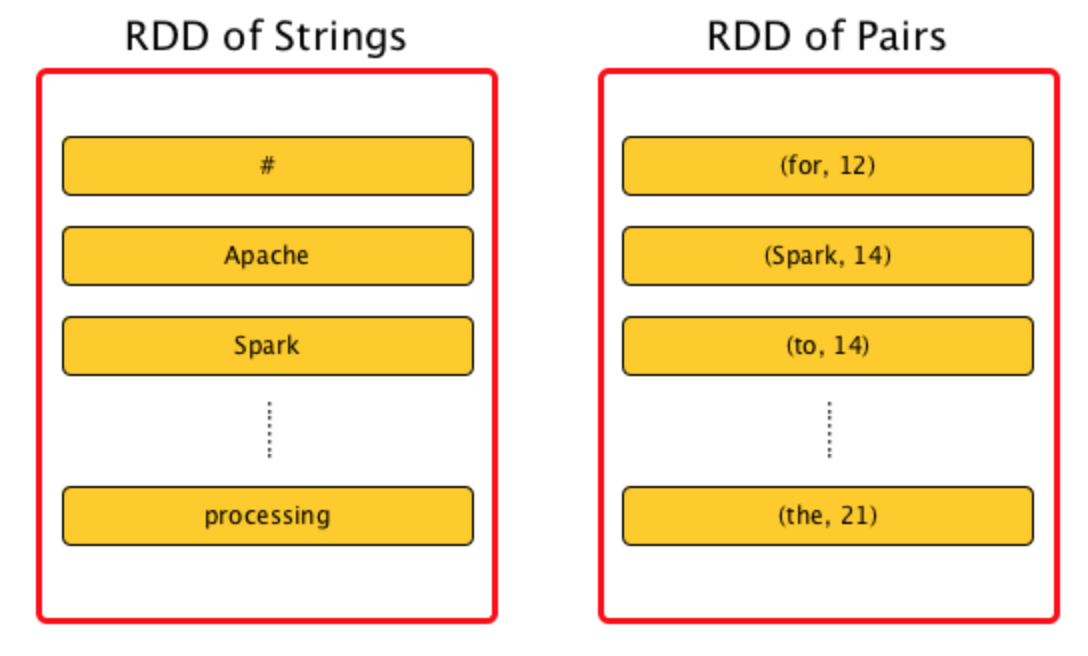
\includegraphics[scale=0.4]{RDD.png}
\caption{RDD結構}
\label{rdd}
\end{figure}

Apache Spark 有著豐富的函數庫,也針對Python, Java, Scala, R等程式語言提供一致的 API,架構如圖\ref{sparkcore},而Apache Spark 當中的核心的為Spark Core,所有API都以此為基礎。Spark Core提供了分散式任務調度、排程和基本I/O ,而主要的程式抽象化結構RDD也是定義在這邊,RDD抽象化是經由Apache Spark 所支援的程式語言整合API呈現的,簡化了寫程式的複雜性。基於Spark Core, Apache Spark 中提供了Spark SQL、Spark Streaing、MLlib以及GraphX 5大類API供使用者進行呼叫。\\\par

\begin{figure}[H]
\graphicspath{{/Users/FUDA/Documents/masterThesis/image/}}
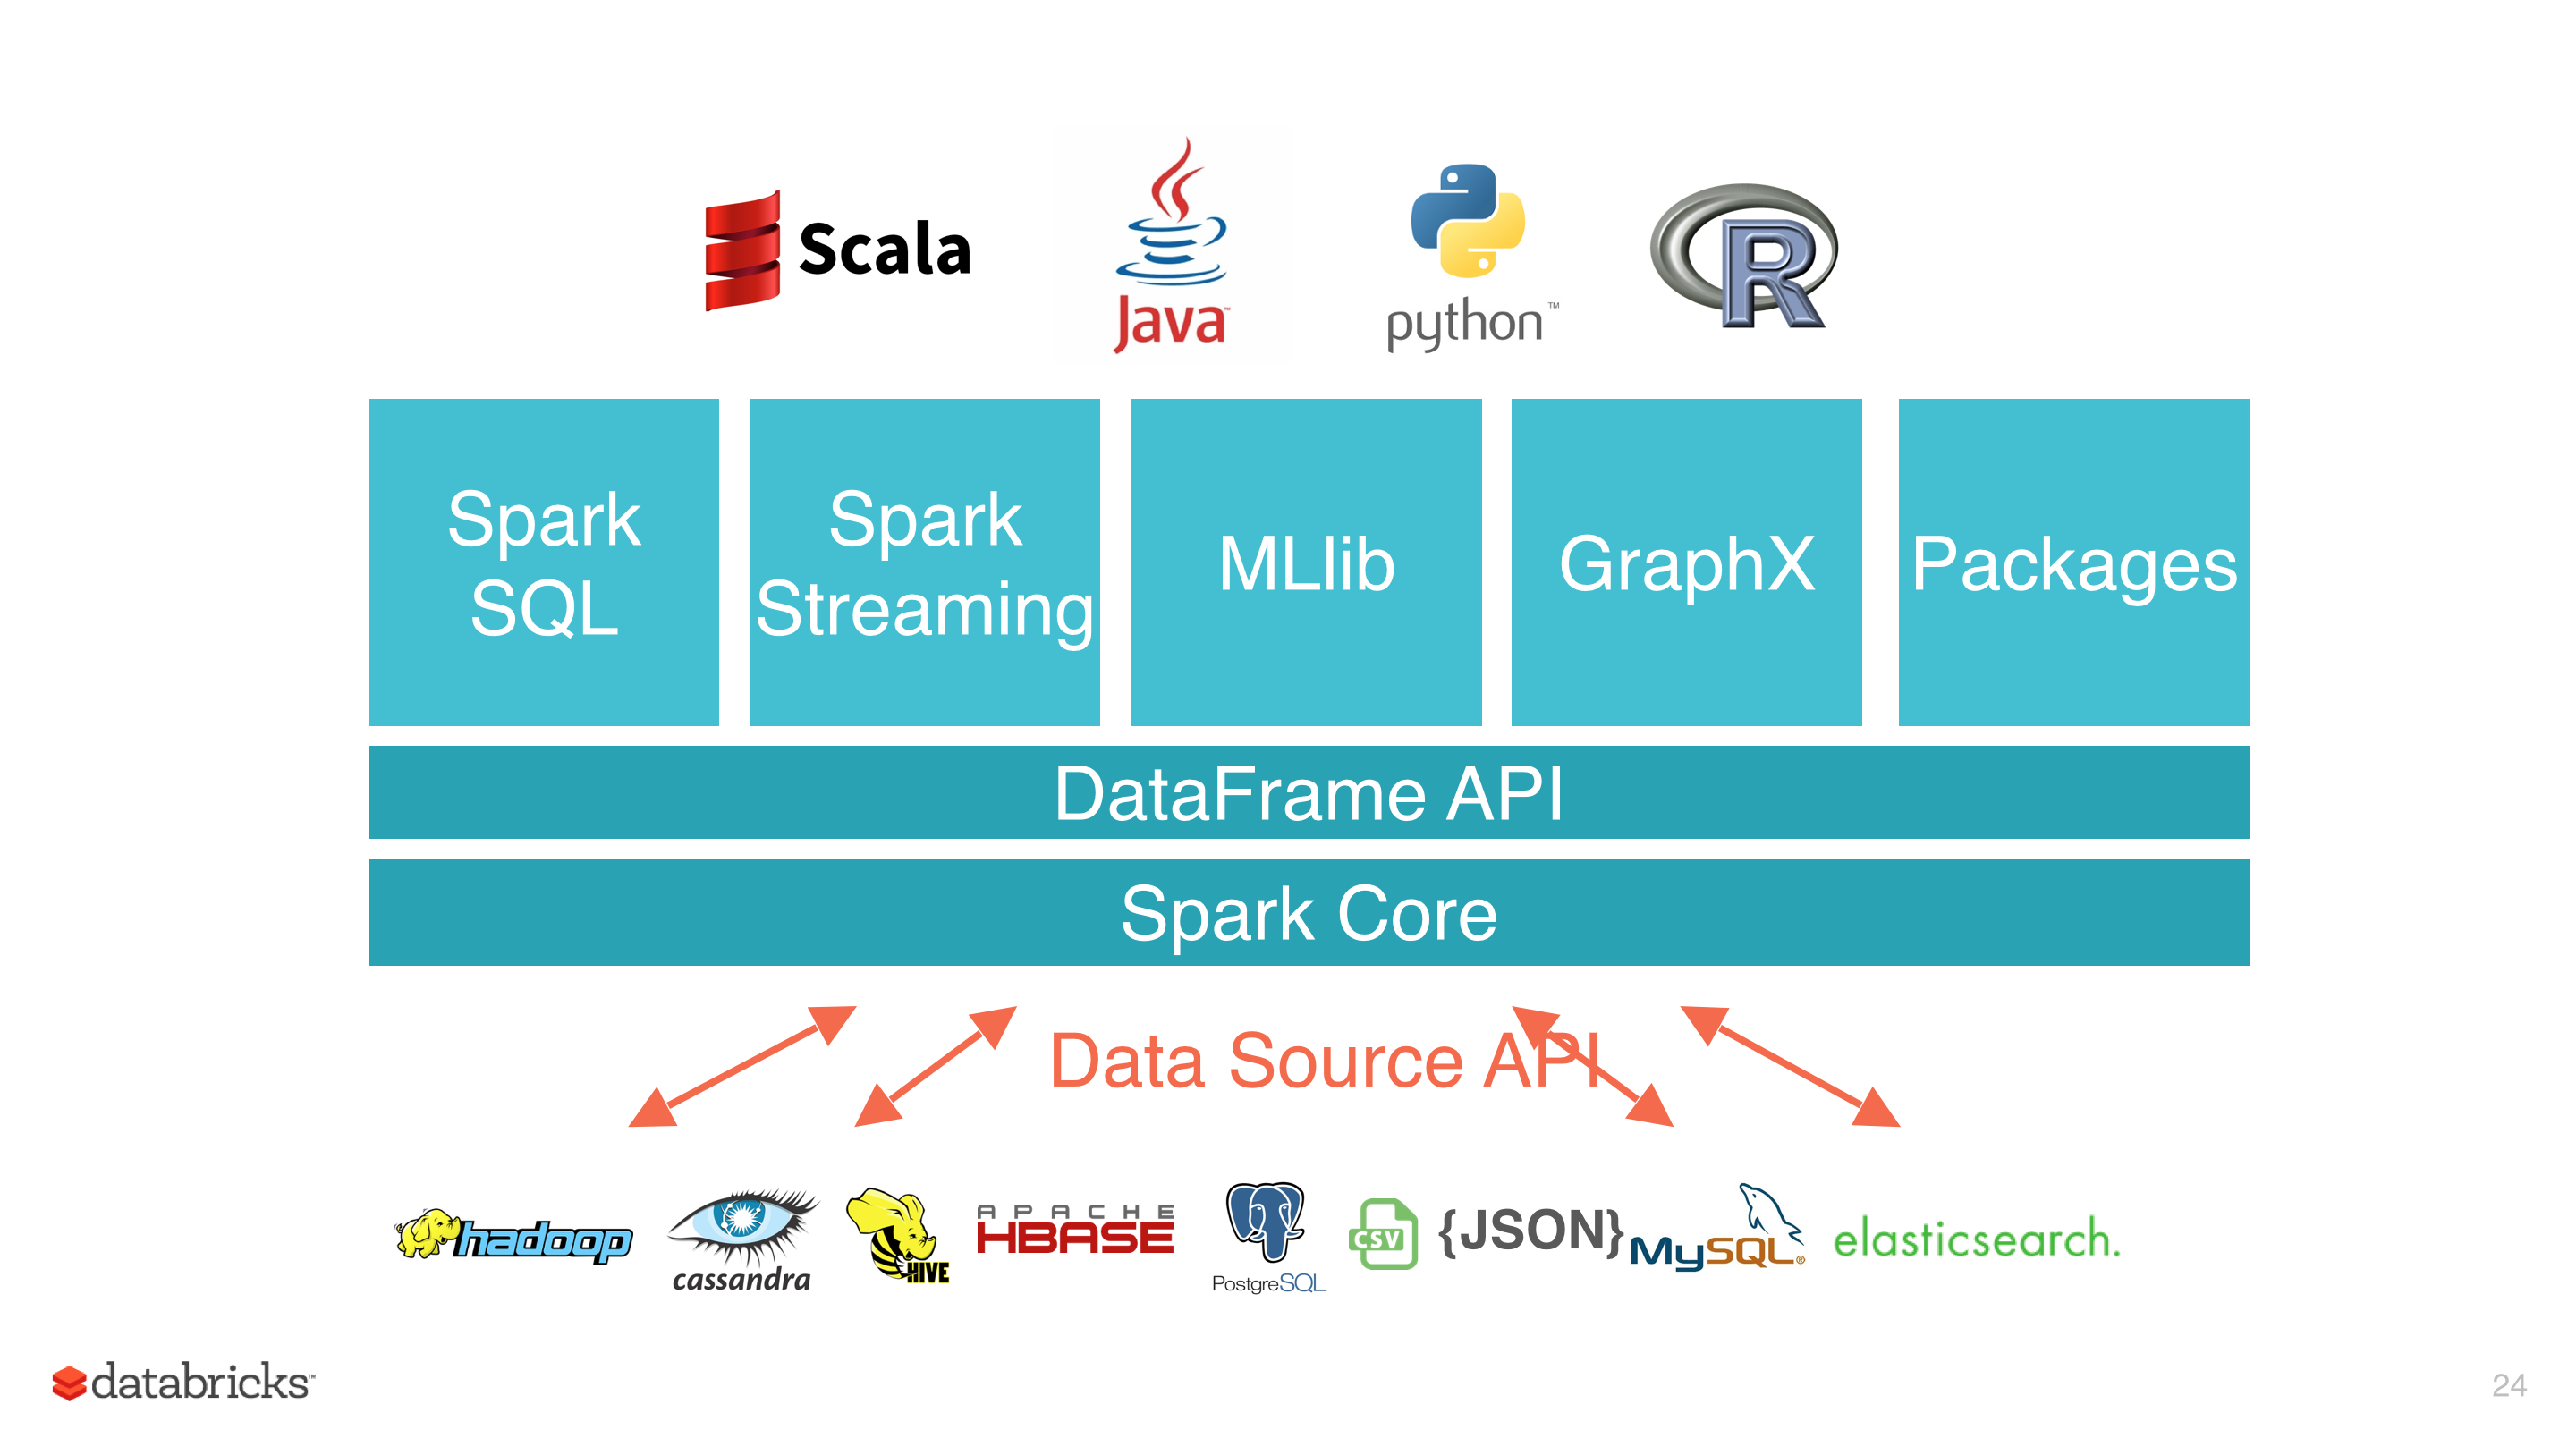
\includegraphics[scale=0.3]{spark.png}
\caption{Apache Spark 核心架構}
\label{sparkcore}
\end{figure}

Spark SQL 在Spark Core上定義了一個叫做 SchemaRDD的資料抽象化概念,提供結構化和半結構化資料的相關支援,另外Spark SQL允許使用者使用SQL遠法做資料查詢,也允許程式開發人員將SQL查詢與其他RDD所支援的資料處理方式一起使用。
Spark Streaming 是在處理即時串流資料的元件,例如web server所產生的紀錄,或是服務狀態的改變,Spark Streaming 擷取了微批次(Micro Batch)的資料並對資料執行RDD的轉換。所謂的微批次是指將每次處理時間的間隔縮小到數秒內,甚至是毫秒等級,雖然也是批次處理,但由於時間間隔變短,感覺起來會趨近於即時處理的效果。Spark Streaming的處理是針對每一個微批次做資料操作,如圖\ref{microbatch}所示:
\begin{figure}[H]
\centering
\graphicspath{{/Users/FUDA/Documents/masterThesis/image/}}
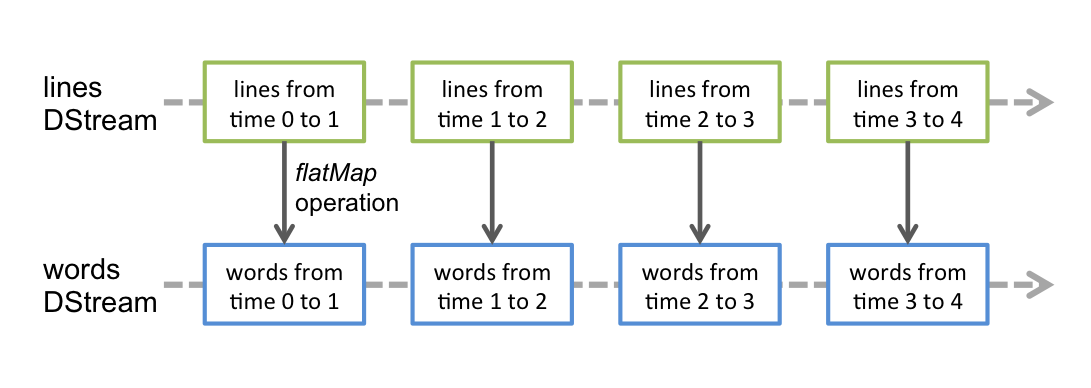
\includegraphics[scale=0.8]{streaming-dstream-ops.png}
\caption{Spark Streaming 微批次資料操作 }
\label{microbatch}
\end{figure}
MLlib是Apache Spark 所提供的機器學習(Machine Learning)函數庫,MLlib可以使用許多常見的機器學習和統計學的演算法,大幅度簡化了機器學習的時間,其中提供了匯總統計、分類、回歸、分群、協同過濾以及最佳化等機器學習及統計分析的演算法。

GraphX是Apache Spark 上的分散式圖形處理框架,此框架可用於表達圖形計算並可以類比Pregel抽象化,GraphX提供了許多處理圖像的操作,例如subgraph和mapVertices以及常見的圖形演算法。
\subsection{大數據XML文件}
所謂的大數據\cite{khan2014big}是指無法以人工管理或是處理的資料集,也可以定義為多來源的結構化或非結構化的資料,而在大數據當中,我們常常用"5V"來描述大數據的特性,這5V分別是規模性(Volume)、價值(Value)、真實性(Veracity)、時效性(Velocity)及多樣性(Variety)。\\\par
5V當中,Volume所代表的是大數據的規模,也就是大數據以傳統的儲存方式已經無法負荷此龐大的資料量或是傳統的資料處理方式已無法對其做運算了;Value是指大數據透過處理後所得到的資料產生的價值;Veracity是指資料的品質,可信度,資料是否可靠,或是結構的完整性;Velocity是指大數據資料產生的速度;Variety是指大數據的資料多樣性,在設計有關大數據的應用的時候,藉由上面五個的特性有助於檢視大數據的特徵。\\\par
XML文件的Veracity真實度這個特性是會有不同的變化的。例如XML文件如果以是否符合DTD規範, well-formed以及vaild的XML文件在真實度Veracity的特性上面就會有不同的變化。我們以兩份well-formed XML來說,上述有提到XML文件的標籤是可以讓使用者自行定義的,所以會造成兩份文件出現相同標籤名稱,意思不同,或是不同標籤名稱,意思相同的狀況,會造成不易判斷的狀況,也有可能在解析完DTD和Schema後發現兩份文件的結構很相似,所以真實度很高的狀況。\\\par
從資料理解性(data understandability)的角度詮釋Veracity的意義來看,假設有兩份XML文件,一份為基準文件B,一份為被量測文件M;我們可以從多個角度去描述「以基準文件觀之,這份被量測文件多少可能是真實的」。例如文件M與文件來源相同,因此文件M應該是真實的。或是文件M與文件B有相同的DTD,因此文件M應該是真實的。或是文件M與文件B的DataGuides相同,因此文件M應該是真實的。這些對於來源相同、DTD相同和DataGuides相同的「想法」,就是用所謂的資料理解性來描述被量測文件M是否是真實的。而由於這樣的想法可以多元且其重要性可能有差異,因此真實性就可以有程度上的區別\\\par

而在這5V當中,本研究要探討的是真實度模型在XML文件的建模與應用,在\cite{veracitymodel}有提出大數據可以由兩個面向來討論,一個是資料理解性,一個是大數據的評價基準,而本研究針對資料理解性面向進行建模,假設有n份基準XML文件以及m份被測量XML文件,使用者可以從多個角度對於XML文件進行真實度計分,XML文件真實度包含的面向極廣,對於真實度的定義每一個人不盡相同,所以本研究建構一個在Apache Spark 叢集上的Veracity真實度模型,使用物件導向程式設計(Object-Oriented Programming,簡稱OOP)的觀念,設計一個維度、屬性以及評分的抽象類別,將基本架構定義完整,做成Veracity Model API且是跑在 Apache Spark 叢集上,將實作細節交給使用者來決定,前面有提到使用者可以從不同的角度來評價XML的真實度評分,以及決定真實度要有多少維度以及多少屬性。並且本研究的模型應用在串流XML上,有別於以往傳統批次文件的處理方式,串流的資料處理方式更符合現代的資料處理架構及場景,而串流XML文件相較於傳統批次處理的XML文件處理方式又有所不同,針對一個大數據串流XML真實度評價模型是一個除了評價資料真實度之外,也可以篩選真實度較高之資料的解決方案。
\subsection{研究動機}
目前在產界與學界中,大數據已經是熱烈討論的議題,而當中的對於5V的研究也已經行之有年。本研究對於大數據的XML文件有以下分析:在Volume的部分因XML時常用於網路資料交換,而隨著大數據應用越來越多。資料交換的頻率以及資料量也會越來越大。而大量的應用也使資料產生的速度加快,是屬於Velocity的部分。資料來源多樣化以及格式上的多樣化則是屬於Variety的部分。大數據當中藏有很多隱藏資訊,藉由資料探勘等技術發現資料的隱藏價值是屬於Value的部分。最後是資料的真實度或是可信度因大數據的資料量極大,使用者或是開發者並不曉得這樣的資料是否可以使用或是否有造假資料參雜其中。\\\par

在上述5V的分析當中,Veracity是本研究關心的焦點,因為所有的資料如果真實度或是可信度不高,在儲存上因為儲存了一堆的無價值資料增加伺服器負擔,分析應用上的結果因資料是真實程度或是可信程度低所以造成結果不具任何價值。本研究將模型應用在串流XML上,以解決串流XML資料因在串流當中結構的不確定性,而導致真實度驗證困難的問題。

\subsection{論文架構}
本論文其餘架構如下。第二章相關研究將介紹XML在分散式系統的處理難處以及問題點,以及在以前是如何做真實度比較。第三章將介紹真實度模型的理論以及設計方法。第四章會實際使用物件導向設計一個真實度模型,以及介紹設計理念。第五章為使用Apache Spark 在串流XML的環境之下間模型實作至叢集當中,並且測試Apache Spark 對於模型計算是否有達到平行化以及建立Dashboard來觀察真實度模型的計算結果以及可用性。第六章將針對模型提出結語以及未來工作方向。
